%%% Hlavní soubor. Zde se definují základní parametry a odkazuje se na ostatní části. %%%

%% Verze pro jednostranný tisk:
% Okraje: levý 40mm, pravý 25mm, horní a dolní 25mm
% (ale pozor, LaTeX si sám přidává 1in)
\documentclass[12pt,a4paper]{report}
\setlength\textwidth{145mm}
\setlength\textheight{247mm}
\setlength\oddsidemargin{15mm}
\setlength\evensidemargin{15mm}
\setlength\topmargin{0mm}
\setlength\headsep{0mm}
\setlength\headheight{0mm}
% \openright zařídí, aby následující text začínal na pravé straně knihy
\let\openright=\clearpage

%% Pokud tiskneme oboustranně:
% \documentclass[12pt,a4paper,twoside,openright]{report}
% \setlength\textwidth{145mm}
% \setlength\textheight{247mm}
% \setlength\oddsidemargin{14.2mm}
% \setlength\evensidemargin{0mm}
% \setlength\topmargin{0mm}
% \setlength\headsep{0mm}
% \setlength\headheight{0mm}
% \let\openright=\cleardoublepage

%% Rozdělování URL na pomlčkách
\usepackage[hyphens]{url}
%% Vytváříme PDF/A-2u
\usepackage[a-2u]{pdfx}

%% Přepneme na českou sazbu a fonty Latin Modern
\usepackage[czech]{babel}
\usepackage{lmodern}
\usepackage[T1]{fontenc}
\usepackage{textcomp}

%% Použité kódování znaků: obvykle latin2, cp1250 nebo utf8:
\usepackage[utf8]{inputenc}

%%% Další užitečné balíčky (jsou součástí běžných distribucí LaTeXu)
\usepackage{amsmath}        % rozšíření pro sazbu matematiky
\usepackage{amsfonts}       % matematické fonty
\usepackage{amsthm}         % sazba vět, definic apod.
\usepackage{bbding}         % balíček s nejrůznějšími symboly
			    % (čtverečky, hvězdičky, tužtičky, nůžtičky, ...)
\usepackage{bm}             % tučné symboly (příkaz \bm)
\usepackage{graphicx}       % vkládání obrázků
\usepackage{fancyvrb}       % vylepšené prostředí pro strojové písmo
\usepackage{indentfirst}    % zavede odsazení 1. odstavce kapitoly
\usepackage{natbib}         % zajišťuje možnost odkazovat na literaturu
			    % stylem AUTOR (ROK), resp. AUTOR [ČÍSLO]
\usepackage[nottoc]{tocbibind} % zajistí přidání seznamu literatury,
                            % obrázků a tabulek do obsahu
\usepackage{icomma}         % inteligentní čárka v matematickém módu
\usepackage{dcolumn}        % lepší zarovnání sloupců v tabulkách
\usepackage{booktabs}       % lepší vodorovné linky v tabulkách
\usepackage{paralist}       % lepší enumerate a itemize
\usepackage{xcolor}         % barevná sazba
\usepackage{float}
\usepackage{subfig}
\usepackage{pdfpages}

%%% Údaje o práci

% Název práce v jazyce práce (přesně podle zadání)
\def\NazevPrace{Dialogový systém pro hlasové vytáčení}

% Název práce v angličtině
\def\NazevPraceEN{A Dialogue System for Voice Dialing}

% Jméno autora
\def\AutorPrace{Borek Požár}

% Rok odevzdání
\def\RokOdevzdani{2021}

% Název katedry nebo ústavu, kde byla práce oficiálně zadána
% (dle Organizační struktury MFF UK, případně plný název pracoviště mimo MFF)
\def\Katedra{Ústav formální a aplikované lingvistiky}
\def\KatedraEN{Institute of Formal and Applied Linguistics}

% Jedná se o katedru (department) nebo o ústav (institute)?
\def\TypPracoviste{Ústav}
\def\TypPracovisteEN{Institute}

% Vedoucí práce: Jméno a příjmení s~tituly
\def\Vedouci{Mgr.\ et Mgr. Ondřej Dušek, Ph.D.}

% Pracoviště vedoucího (opět dle Organizační struktury MFF)
\def\KatedraVedouciho{Ústav formální a aplikované lingvistiky}
\def\KatedraVedoucihoEN{Institute of Formal and Applied Linguistics}

% Studijní program a obor
\def\StudijniProgram{Informatika}
\def\StudijniObor{Obecná informatika}

% Nepovinné poděkování (vedoucímu práce, konzultantovi, tomu, kdo
% zapůjčil software, literaturu apod.)
\def\Podekovani{%
Chtěl bych poděkovat především svému vedoucímu Mgr.\ et Mgr. Ondřeji Duškovi, Ph.D.
za veškerou pomoc a trpělivost s teoretickou částí práce. Dále pak RNDr. Janu Cuřínovi, Ph.D. 
a RNDr. Martinu Čmejrkovi, Ph.D. za asistenci s praktickou částí práce. Nakonec také všem 
uživatelům, kteří se zapojili do testování.
}

% Abstrakt (doporučený rozsah cca 80-200 slov; nejedná se o zadání práce)
\def\Abstrakt{%
Dialogové systémy jsou dnes velmi populární, jak mezi uživateli chytrých
telefonů či reproduktorů, tak mezi firmami, které je využívají ke snížení
množství potřebných pracovníků zákaznické podpory.
Hlavním cílem práce je představení vlastní implementace dialogového systému
pro hlasové vytáčení v~češtině. Systém je implementován jako aplikace
pro mobilní telefony s~operačním systémem Android, která k~rozpoznání
a syntéze řeči využívá služby Google. Řízení dialogu zajišťuje instance asistenta
IBM Watson implementovaná autorem za využití služeb poskytovaných IBM.
Porovnání se seznamem kontaktů provádí nově implementovaná komponenta běžící
v~cloudu. Ta entity rozpoznané pomocí asistenta porovnává se seznamem kontaktů
uživatele, navíc bere v~úvahu i původní uživatelův vstup.
Aplikace je psána v~jazyce Kotlin, porovnávací komponenta
v~jazyce Python. Úspěšnost systému byla vyhodnocena
na základě zkušeností reálných uživatelů. Celkově se 15 uživatelů pokusilo
zahájit 91 hovorů, z~čehož 51 se podařilo, což znamená úspěšnost \(56\,\rm \%\).
Podle zpětné vazby jsme navrhli možná vylepšení, která rovněž popisujeme.
}
\def\AbstraktEN{%
Dialogue Systems are getting more and more popular, among users and companies alike.
Users enjoy using smartphones and smart speakers; companies can hire fewer workers in support
centres. The main goal of this thesis is to implement a dialogue system for voice dialing in
the Czech language. The system is implemented as a mobile application for phones with
the Android operating system which utilizes Google STT/TTS for voice communication
with the user. The dialogue is handled by an instance of IBM Watson Assistant, which we
have developed for the domain. Entities found by the assistant are matched against the
user's contact list using a newly implemented matching component. This component takes
the raw textual input into account to improve on the entities recognized by Watson Assistant.
The application is implemented in the Kotlin language, the matching component in Python.
The system was evaluated with real users. 15 test users tried to make 91 phone
calls and 51 of them were successful, which means a success rate of \(56\,\rm \%\). Based on the
user feedback we came up with ideas for improvements.
}

% 3 až 5 klíčových slov (doporučeno), každé uzavřeno ve složených závorkách
\def\KlicovaSlova{%
{dialogové systémy}, {hlasová aplikace}, {porozumění jazyku}, {zpracování přirozeného jazyka}
}
\def\KlicovaSlovaEN{%
{dialogue systems}, {voice application}, {language understanding}, {natural language processing}
}

%% Balíček hyperref, kterým jdou vyrábět klikací odkazy v PDF,
%% ale hlavně ho používáme k uložení metadat do PDF (včetně obsahu).
%% Většinu nastavítek přednastaví balíček pdfx.
\hypersetup{unicode}
\hypersetup{breaklinks=true}

%% Definice různých užitečných maker (viz popis uvnitř souboru)
\include{makra}

%% Titulní strana a různé povinné informační strany
\begin{document}
\include{titulka}

%%% Strana s automaticky generovaným obsahem bakalářské práce

\tableofcontents

%%% Jednotlivé kapitoly práce jsou pro přehlednost uloženy v samostatných souborech
\chapter*{Úvod}
\addcontentsline{toc}{chapter}{Úvod}

Mluvené slovo je pro člověka nejjednodušším způsobem komunikace. Je to
způsob rychlý, efektivní a nevyžaduje použití hmatu či zraku. Tyto smysly
tak zůstávají volné pro využití jiným způsobem, například můžeme zároveň
řídit auto či vařit oběd. V případě mateřského jazyka je navíc použita
syntaxe, kterou se učíme od narození, tedy taková komunikace nevyžaduje
nějakou speciální znalost, jako seznam příkazů programu nebo funkce
ovládacích prvků.

Přirozený jazyk proto vypadá jako v mnoha směrech ideální médium pro výměnu
informací mezi uživatelem a strojem. Proč ho tedy nepoužíváme víc už dávno?
Extrahovat z něj význam tak, aby mohl být pochopen strojem, není vůbec
jednoduché. Většího průlomu v tomto směru se podařilo dosáhnout až s příchodem
technologií strojového učení, které jsou schopny se složité zákonitosti
jazyka \uv{samy} naučit. Ani to však není samospásné, pro naučení modelu,
který porozumí jazyku, je stále potřeba mnoho práce, dat a počítačového
výkonu. Pomyslně na druhém konci komunkace pak leží problém vygenerovat
odpověď zpět uživateli, který není o moc jednodušší.

Pokrok v těchto směrech dal možnost vzniku a rozšíření
\textit{hlasových asistentů}, které dnes již skoro každý nosí ve svém
chytrém telefonu a mnozí je navíc mají doma v podobě \uv{chytrého}
reproduktoru. Jak již bylo zmíněno, vývoj takové služby je náročný v mnoha
směrech, proto jsou asistenti obvykle dostupní jen v nejpoužívanějších
jazycích, jako je angličtina, španělština nebo němčina. Nakolik je autorům
známo, jediným asistentem podporujícím češtinu je \textit{IBM Watson Assistant}
(dále WA) a to pouze v textové podobě.

Cílem této práce je vytvořit hlasového asistenta v češtině, který bude schopný
odpovídat na pozdravy a především zavolat kontakty ze seznamu v telefonu.
Toho bude dosaženo propojením WA s vlastní komponentou
pro porovnání se seznamem kontaktů, \textit{Google STT/TTS}
(rozpoznání a generování mluvené řeči) a funkcionalitou telefonu. Výhodou
je relativně jednoduché rozšíření asistenta přidáním variant dialogu do WA
a ošetřením speciálních odpovědí z WA v mobilní aplikaci, aby iniciovaly
například otevření jiné aplikace nebo rozsvícení svítilny.

V příštích několika kapitolách je uvedeno shrnutí teorie související
s tématem, následuje popis vlastní implementace a zkušenosti uživatelů,
kteří aplikaci zkoušeli. V závěru je rozebrána úspěšnost splnění
vytyčených cílů.

\chapter{Dialogové systémy}\label{chapter-theory}

Toto je teoretický úvod představující důležité pojmy.
Jak název napovídá, dialogové systémy vedou dialog s uživatelem. Jsou to
tedy jakékoliv programy (nebo skupiny programů) využívající
pro komunikaci přirozený jazyk, obvykle ve formě textové nebo hlasové.
Vyčerpávající shrnutí tohoto tématu, souvisejících problémů a metod
jejich řešení podávají \citet{jurafsky_slp_2020}. Za zmínku jistě stojí
i kniha \textit{Conversational AI} \citep{mctear_conversational_2020} nebo
článek \textit{Neural Approaches to Conversational AI} \citep{gao_neural_2019},
kde se autoři zabývají aplikací strojového učení.

\section{Dělení systémů}
Dialogové systémy můžeme dělit dle mnoha různých specifik. Asi vůbec
nejzákladnějším je dělení na systémy \textit{zaměřené na plnění úkolů}
(rozšířený je anglický termín \textit{task-oriented}), jejichž úkolem
je dosáhnout nějakého uživatelova cíle; a \uv{\textit{tlachací}} (anglicky
\textit{chitchat}), jejichž úkolem je jen vést s uživatelem smysluplnou
konverzaci \citep[strana 6]{gao_neural_2019}.

\textit{Doménou} systému se rozumí téma, kterému by se měl být schopen
věnovat. Podle toho, zda to dokáže jen u jednoho, nebo u více různých,
můžeme systém nazývat \textit{jednodoménový} nebo \textit{vícedoménový} \citep[strana 47]{gao_neural_2019}.

Dále můžeme systémy dělit podle toho, kdo řídí dialog. Dotaz či změnu tématu
může iniciovat vždy pouze uživatel a systém jen odpovídat, nebo naopak, nebo
se mohou v iniciativě střídat \citep[strany 495-496]{jurafsky_slp_2020}. Implementace posledního jmenovaného je samozřejmě
nejkomplikovanější.

Posledním dělením, které uvedeme, je podle kanálů komunikace, tedy
v jaké prvotní formě je informace mezi uživatelem a systémem předávána.
Obvykle je forma na obou stranách stejná, může se však i lišit. Mezi
nejčastější patří text, mluvená řeč a obraz (ať už statický nebo
dynamický), ale existují již i humanoidní roboti schopni vyjadřovat emoce pomocí
mimiky, jednoho takového popisují \citet{faraj_facially_2021} ve svém článku.

My se nadále budeme zabývat systémem zaměřeným na plnění úkolů v rámci jedné
domény, který má jako vstup i výstup mluvenou řeč, protože do této kategorie
naše implementace spadá.

\section{Problémy ve zpracování dialogu}

Při trochu podrobnějším pohledu na většinu rozhovorů zjistíme, že nejsou
tak jednoduché a přímočaré, jak si představujeme \citep[sekce 24.1]{jurafsky_slp_2020}. To dále ztěžuje
veškeré strojové zpracování. Některé komplikace umíme řešit jen do určité
míry, některé zatím vůbec. Vezměme si například takovýto smyšlený dialog:

\begin{code}
    A: Dal bych si.. hmmm.. majoránku, tedy pardon! Marokánku.
    B: S sebou, nebo..
    A: Vlastně ne! Raději cheesecake.
\end{code}

Jistě si dokážeme představit, že by mohl proběhnout a připadal by nám
relativně normální. S čím se však musejí aktéři vypořádat? Mluvčí A se
nejdříve rozmýšlí a druhý to musí pochopit a počkat. Poté se rozhodne
a něco řekne, mluvčí B to pochopí, ale vzápětí musí své pochopení
poupravit, protože A se jen přeřekl a opravuje se. Když se B konečně
dostane ke slovu, začne mluvit, ale hned musí zase skončit, protože
A mu skáče do řeči s další opravou -- přeje si cheesecake. Pokud by
však B neznal toto anglické slovo (systém naučený rozpoznávat češtinu
by nemusel), v hlučnějším prostředí by pravděpodobně pochytil spíše
něco jako \uv{čistej}. Nejběžnější problémy, se kterými se v tomto
směru potýkáme, rozebereme v následujících třech podsekcích.

\subsection{Začátek a konec promluvy}

Prvním problémem je jak vůbec zjistit, kdy uživatel dialog začal, kdy
skončil svůj \textit{tah} (souvislou promluvu, po které obvykle očekává odpověď),
a kdy skončil celý dialog \citep[strana 494]{jurafsky_slp_2020}.
Jako lidé jsme většinou schopni začátek dialogu rozpoznat tím, že se na
nás druhý podívá či nás osloví. Pohled u stroje s pouze zvukovým vstupem
detekovat schopni nejsme, oslovení dnešní technologie již dokáží. Většinou
definujeme jedno nebo několik slov, které stroj chápe jako začátek dialogu,
tzv. \textit{wake-up words}. Součást systému detekující tato slova musí být velmi
výpočetně úsporná, protože je nutné, aby běžela neustále. Dnes jsou obvykle
využívány komponenty založené na hlubokém učení, jako třeba Howl
\citep{tang_howl_2020}.
Běžným způsobem je ale stále zahájení dialogu stiskem tlačítka či něčím
podobným.

Zahájení jsme tedy detekovali, ale jak poznat konec? Za konec tahu je
většinou považována delší pauza, v takovou chvíli systém vyhodnotí odpověď
a začne odpovídat. Problém je, pokud jsme konec tahu detekovali špatně a
v průběhu systémové odpovědi začne uživatel opět mluvit. V lidské konverzaci
se to stává běžně a umíme se s tím jednoduše vypořádat, protože jsme schopni
zároveň mluvit a poslouchat. U strojů to však problém je a je náročné ho řešit,
běžnou praxí asistentů
je proto začít znovu poslouchat až po ukončení jejich promluvy.

Existují však již i \textit{inkrementální} dialogové systémy, které
vstup zpracovávají průběžně a detekují konec tahu i jinými způsoby.
Možné způsoby (často využívané i člověkem) popisují \citet{turn_taking_taxonomy_2015},
\citet{khouzaimi_turn-taking_2016} pak ve své práci navrhuje
možnou architekturu inkrementálních systémů a způsob jejich učení.

Úplný konec dialogu většinou detekujeme buď explicitně, zvolenými klíčovými
slovy (třeba \uv{konec}) či frázemi (rozloučení); nebo implicitně, pokud
systém splní uživatelův cíl či uživatel již neodpoví.

\subsection{Zpracování zvuku}

Při převodu mluveného slova na text narážíme na problémy spousty nepřesností \citep[sekce 4.1]{glass_challenges_1999}.
Přepis nám ztěžuje okolní hluk, který dokážeme automaticky odfiltrovat jen do určité míry
a obtížně. Navíc pokud dojde k chybě v nějakém slově, můžeme se ji sice snažit
z kontextu nějak zpětně opravit, ale opět je to složitá práce navíc. Člověk
tyto drobné opravy na základě kontextu dělá podvědomě a bravurně.

Dále se potýkáme s různou výslovností různých lidí, přeřeky, opravami
či výplňovými zvuky, kdy se mluvčí rozmýšlí, co chce říct dál. Zvláště
pokud se něco takového vyskytne uprostřed slova, může být obtížné dát
strojově dohromady výsledek promluvy.

\subsection{Očekávané znalosti, domýšlení}

Při běžné komunikaci člověk od druhého očekává určitou míru přehledu o světě
-- minimálně fakta typu \uv{Slunce je na obloze} považujeme za samozřejmá.
Předáváním těchto obecných znalostí dialogovým systémům se ve svém článku
zabývají \citet{young_augmenting_2018}.

Také očekáváme, že druhý bude schopen pochopit význam zájmen, odkazů
a obecně věcí nevyjádřených přímo. Více výrazů odkazujících na jednu věc
označujeme \textit{koreference}, podrobnější popis tématu dávají
\citet[kapitola 21]{jurafsky_slp_2020}.


\section{Konstrukce dialogových systémů}

Tradiční přístup implementace bychom mohli označit jako postupný. Čítá několik
komponent, kde každá zajišťuje část práce nutné k porozumění uživateli a
zodpovězení jeho prohlášení \citep[sekce 4.1]{gao_neural_2019}. Takovou konstrukci budeme nazývat \textit{pipeline}.
Tento přístup dobře ilustruje, co všechno vlastně
člověk podvědomě při komunikaci dělá. Druhý přístup reprezentují tzv. \textit{end-to-end}
systémy využívající metod strojového učení, které umožňují nahrazení až
několika komponent jedním modelem \citep[sekce 4.6]{gao_neural_2019}. Taková implementace první uvedený v mnohém
předčí, ale v praxi se příliš nevyužívá z důvodu náročnosti na trénovací data.

Již jsme zmínili, že vícekrokové systémy mají několik komponent, které na sebe
navazují, jedna obvykle určitým způsobem využije výstup z předchozí jako svůj
vstup. Nejčastěji se používá rozdělení na šest částí, kterým se podrobněji
budeme věnovat v následujících podsekcích. Jsou to: převod textu na řeč (v podsekci~\ref{stt}),
extrakce významu (\ref{nlu}), udržování stavu (\ref{dst}), rozhodnutí o dalším kroku (\ref{dp}),
vytvoření odpovědi v přirozeném jazyce (\ref{nlg}) a syntéza hlasu (\ref{tts}). První
a poslední u textových systémů odpadají.

\subsection{Převod mluvené řeči na text}\label{stt}

Zkráceně značíme nejčastěji \textit{STT} z anglického \textit{speech-to-text}.
Jak název napovídá, úkolem této komponenty je převést zvukový projev na text.
Dříve byly k tomuto účelu využívány především \textit{skryté
    Markovovy modely (hidden Markov models, HMM)}. Tyto modely se nazývají skryté,
protože jejich vnitřní stavy nemohou být pozorovány, vidíme pouze výstup.
Jsou postaveny na \textit{Markovových řetězcích}, jejichž základním předpokladem
je, že v sekvenci stavů pravděpodobnost příštího závisí jen na stavu aktuálním,
nikoliv žádném předchozím, jak uvádí například \citet[strana 4]{brooks_handbook_2011}.
Jejich výhodou je, že jsou poměrně jednoduché a nenáročné na výpočetní výkon.

Jako v mnoha jiných odvětvích, i zde přišly ke slovu neuronové sítě, které HMM
ve většině směrů překonaly. V dobrých podmínkách jsou schopny provést přepis
téměř bezchybně \citep{zhang_pushing_2020}. Opět však narážíme i na jejich slabé stránky,
totiž vysokou náročnost na množství trénovacích dat a výpočetní výkon.

O obecných problémech typu okolního hluku či různé výslovnosti jsme se
již zmiňovali. Zde ještě dodáme, že komplikací může být i nedostatečná kvalita
nahrávky. Mimo jiné z těchto důvodů výstupem často nebývá jen jedno
slovo či věta, nýbrž několik spolu s \textit{jistotou}, kterou model této
variantě přiřadil.

\subsection{Extrakce významu}\label{nlu}

\subsubsection{Obecný význam}
Nyní když máme textovou reprezentaci výpovědi, budeme se z ní snažit nějak
jednodušeji vyjádřit podstatné části. Této komponentě se obvykle říká
\textit{porozumění jazyku (natural language understanding, NLU)}. V jistém
smyslu je její úkol nejnáročnější, neboť jazyky mají mnoho nejasností,
víceznačností a nuancí obecně. Výstupem této komponenty je často opět
seznam reprezentací s hodnotou, nakolik si je systém tou konkrétní
interpretací jistý \citep[sekce 4.3]{gao_neural_2019}.

K získání oné jednodušší reprezentace můžeme využít \textit{dialogových aktů}
(\textit{DA}) \citep[strana 494]{jurafsky_slp_2020}. Ty pak
často popisujeme například trojicemi \textit{úmysl}--\textit{slot}--\textit{hodnota},
ale používány jsou různé reprezentace. Několik jich popisují a
metodologii pro převod z nich do podmnožiny
ISO standardu navrhují \citet{mezza_iso-standard_2018}.

Použití trojic můžeme ilustrovat na úryvku \uv{v deset hodin}, který bychom
přeložili na trojici
informovat--čas--10:00. K získání relevantních trojic můžeme využít ručně
psané \textit{regulární výrazy} vyhledávající vzorce v textu, tento přístup
je však dost náročný. Pro rozumnou funkcionalitu takových výrazů musíme napsat
stovky. Dnes obvykle lepší alternativou jsou opět modely využívající strojové
učení. Aplikaci hlubokých neuronových sítí na tento problém
popisují \citet{liu_multi-task_2019}.

\subsubsection{Jména a názvy}
Důležitou součástí je \textit{rozpoznávání jmenných entit} (anglicky
\textit{named entity recognition, NER}),
kde cílem je rozpoznat v textu názvy, které jako slova sama o sobě nemají
význam, pokud nevíme, že jde o název. Zajímají nás jak jména lidí, tak
geografických objektů či čehokoliv jiného, v závislosti na cílové doméně.

K jejich nalezení se opět často používají modely strojového učení, pro češtinu
jeden takový popsali \citet{ekstein_czech_2019}. Na pomoc či další zpracování
můžeme využít metriky vzdálenosti mezi textovými řetězci,
jako je \textit{Levenshteinova vzdálenost}, pravděpodobně představena autorem v
článku roku 1965 \citep{Levenshtein1965BinaryCC}. Ta říká, kolik nejméně úprav
musíme u jednoho řetězce udělat, abychom dostali druhý, tedy zjednodušeně řečeno
jak moc jsou si dva řetězce podobné. Trochu problém nastává u krátkých slov,
protože u nich i velmi málo úpravami můžeme dostat slovo kompletně rozdílné.

\subsection{Udržování stavu}\label{dst}

Od systému samozřejmě budeme vyžadovat určitou paměť. Pokud řekneme, že
chceme někomu zavolat, pak dostaneme otázku komu, a pak ji zodpovíme, očekáváme,
že systém si bude ještě pamatovat, že chceme volat. Tato komponenta je
značena \textit{DST} z anglického \textit{Dialogue State Tracker}. V případě
zmíněné reprezentace pomocí trojic paměti docílíme obvykle tak, že si pro každý
slot pamatujeme hodnotu. Buď jednu, kterou v případě detekce jiné ihned přepíšeme,
nebo si pro každý slot pamatujeme pravděpodobnostní rozložení více hodnot, které
průběžně upravujeme. Téma hezky shrnují \citet{williams_dialog_2016}.
Paměť nesmíme zapomenout v určitých případech
resetovat, například když uživatel změní celý svůj cíl, jím dříve
zmíněné hodnoty se stávají irelevantními.

\subsection{Rozhodnutí o dalším kroku}\label{dp}

Máme uživatelovu aktuální výpověď a relevantní historii dialogu, nyní potřebujeme
rozhodnout, jak zareagujeme. Můžeme ručně napsat pravidla, na základě kterých
se rozhodneme o odpovědi. U systémů zaměřených na plnění úkolů je častou
strategií snaha zjistit uživatelův cíl a následné získání informací potřebných
k tomuto cíli (například pokud máme zarezervovat let, potřebujeme vědět kdy,
odkud a kam), jinými slovy vyplnění potřebných slotů \citep[strany 504-506]{jurafsky_slp_2020}. Rozhodovacích pravidel
však potřebujeme mnoho a zvláště u větších systémů může být výsledný proces dost
zmatený. I zde jsou dnes využívány statistické modely a různé druhy strojového
učení (hodí se zmínit především \textit{zpětnovazební} \citep{su_reward_2015}). Výstupem této komponenty
bývá opět určitý mezistupeň, jednodušší reprezentace nesoucí význam. Využít
můžeme již zmíněné trojice úmysl--slot--hodnota.

\subsection{Vytvoření odpovědi v přirozeném jazyce}\label{nlg}

Z interní reprezentace významu nyní potřebujeme vytvořit odpověď v přirozeném
jazyce, kterou pochopí libovolný uživatel. Můžeme využít \textit{šablon}, do
kterých doplníme vynechané části dle stavu dialogu \citep[strana 508]{jurafsky_slp_2020}. Například pokud bychom
se zabývali rezervacemi letů, mohla by naše potvrzovací šablona vypadat jako
\uv{Přejete si odlétat \{den\} v \{čas\} z \{letiště\}?} a dle stavu dialogu
bychom ji doplnili na \uv{Přejete si odlétat zítra v 10:00 z Londýna Lutonu?}.
Přidáním více variant pro každou šablonu dosáhneme i určité autenticity dialogu.
Z variant pak můžeme volit náhodně, sekvenčně či heuristicky podle uživatelova
vyjadřování, například pokud se vyjadřuje nespisovně, mohli bychom se také
chtít vyjadřovat nespisovně. Opět narážíme na pracnost tohoto přístupu, šablon
totiž i pro jednotlivou doménu musíme vytvořit desítky a více. Přesto mohou
posloužit až překvapivě dobře. Dalšími možnostmi je použít formálních gramatik
\citep{teich_grammars_1999} či i zde strojového učení \citep{wen_stochastic_2015}.

\subsection{Převod textu na řeč}\label{tts}

Obdobně jako u převodu opačným směrem, značíme \textit{TTS} (z \textit{text-to-speech}).
Důležitými pojmy
při popisu řeči jsou \textit{fón}, což je v zásadě jakýkoliv zvuk nehledě na
význam; a \textit{foném}, což je nejmenší část jazyka,
pomocí které jsme schopni význam rozlišit \citep[kapitola 1]{li2020universal}. Především jejich analýza pomáhá
při snaze o počítačovou syntézu řeči, pokud nevyužíváme strojového učení.

Důkazem může být například
\textit{konkatenační} přístup k syntéze hlasu, kdy nahrajeme mluvu člověka,
nahrávku rozdělíme na \textit{difóny} (dva za sebou jdoucí fóny) a ty pak
zpět \uv{slepíme} v požadovaném pořadí \citep{OSHAUGHNESSY198855}. V této základní variantě dostaneme
hlas, který bude znít značně roboticky (mimo jiné kvůli absenci intonace či
přízvuků), ale uživatel z něj dokáže pochopit význam. Při dostatečném množství
vzorových dat a aplikaci dalších vylepšení však dostáváme již velmi dobré
výsledky.

Dalším přístupem je opět využití HMM a jiných modelů strojového učení.
Google TTS poskytuje několik hlasů využívajících různé technologie. Jak uvádí \citep{google_tts},
jejich \textit{standardní} hlasy jsou založené na parametrickém přístupu,
který používá \textit{vocodery}. Jeden
nazvaný \textit{Vocaine} představuje \citet{vocaine_2015}. Zbylé nabízené
hlasy jsou založené na modelu \textit{WaveNet} \citep{oord_wavenet_2016},
který využívá hlubokou neuronovou síť. Zajímavé je srovnání posouzené
přirozenosti řeči na obrázku~\ref{img-wavenet}, kde se WaveNet dostává velmi blízko
lidskému hlasu. Za zmínku jistě stojí ještě \textit{Tacotron} \citep{wang2017tacotron},
odkazy na další články ohledně jeho vylepšování shrnuje webová
stránka \citep{google_github_tacotron}, kde můžeme najít i ukázky různých verzí.
Bohužel se nám nepodařilo zjistit, který z těchto přístupů je využíván
na Androidu, ale protože hlasy používající WaveNet nabízí Google jako svým
způsobem prémiové, domníváme se, že půjde o hlasy standardní.

\begin{figure}[h]
    \centering
    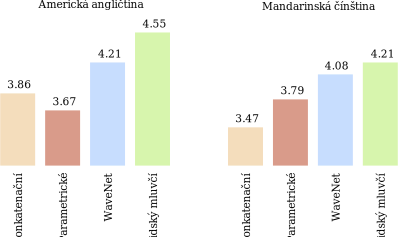
\includegraphics[angle=90, width=0.98\textwidth]{../img/wavenet-comparison.pdf}
    \caption{Porovnání průměrného hodnocení přirozenosti řeči na stupnici 1-5, převzato z dokumentace
        \citet[upraveno a přeloženo autorem]{google_tts}.}
    \label{img-wavenet}
\end{figure}

\chapter{Konstrukce dialogových systémů}

Začneme popisem obecné terminologie, následovat bude krátké shrnutí dvou
nejběžnějších přístupů ke konstrukci. Tradiční je přístup, který bychom
mohli označit jako postupný. Taková konstrukce čítá několik komponent, kde
každá zajišťuje část práce nutné k porozumění uživateli a zodpovězení jeho
prohlášení. Ten uvedeme jako první, neboť dobře ilustruje, co všechno vlastně
člověk podvědomě při komunikaci dělá. Dále uvedeme tzv. \textit{end-to-end}
systémy využívající metod strojového učení, které umožňují nahrazení až
několika komponent jedním modelem. Tento přístup první uvedený v mnohém
předčil, ale je běžnou praxí obě konstrukce kombinovat.

\section{Terminologie}

Během dialogu se střídají promluvy dvou a více stran. Každou takovou promluvu
budeme označovat jako \textit{tah}. Při snaze zaznamenat jednodušeji význam
vysloveného obvykle používáme trojice
\textit{úmysl}--\textit{slot}--\textit{hodnota}. Pro ilustraci například
úryvek \uv{v deset hodin} bychom mohli přeložit na trojici
informovat--čas--10:00.
\chapter{Vlastní vývoj}

Na začátku této kapitoly rozebereme zvolenou platformu a programovací jazyky.
Další části budou věnovány popisu komponent programu, konkrétně aplikaci pro
mobilní telefony s operačním systémem Android, vytvoření instance WA pro řízení
dialogu (s popisem získání nejběžnějších českých jmen pro trénink) a komponenty
pro porovnání entit nalezených pomocí WA se seznamem kontaktů běžící v cloudu.

\section{Platforma a programovací jazyky}

\subsection{Platforma a jazyk mobilní aplikace}
Pro mobilní aplikace máme v dnešní době v zásadě dvě možnosti, iOS nebo Android.
Zvolili jsme Android, neboť je celkově otevřenější, autoři telefon s tímto
operačním systémem vlastní a mají tedy alespoň uživatelské zkušenosti. IBM navíc
poskytuje vývojový balíček (\textit{SDK}) pro použití WA v programovacím
jazyku Java, který je použitelný i v Androidu.

Z hlediska programovacího jazyka padla volba na Kotlin. Existují různé frameworky
schopné zkompilovat pro Android program psaný téměř v libovolném programovacím
jazyce, ale většina nakonec musí používat nějakou další překladovou vrstvu.
Kotlin je jeden z jazyků, ve kterém lze psát nativní aplikace pro Android. Je
totiž založený na Javě a dokonce umožňuje interoperabilitu s ní, což umožnilo
využití zmíněného SDK. Jeho výhoda oproti Javě je, že je celkově modernější,
psaní a čtení programů v něm je díky přehlednější syntaxi jednodušší a kratší,
navíc je doporučený samotnou firmou Google jakožto vedoucím vývoje operačního
systému Android. Další vlastností, na kterou při výběru nebyl brán tak velký
zřetel, ale nakonec se ukázala jako relativně zásadní, je podpora koprogramů
(pravděpodobně známější pod anglickým názvem \textit{coroutines}).

\subsection{Volba asistenta a jeho inicializace}
Asistentů existuje na trhu mnoho, jen jeden však aktuálně oficiálně plně
podporuje český jazyk -- Watson Assistant od IBM. Proto zde volba jednoduše
padla právě na něj.

Inicializace WA lze provést v interaktivním prostředí v prohlížeči. Toto
prostředí je však v mnohém omezené. V našem případě jsme například potřebovali
vložit stovky entit pro trénování rozpoznání. Přenést je do WA přes prohlížeč
by bylo absurdně náročné, navíc složitě replikovatelné. Sáhli jsme proto opět
po SDK, pomocí kterého můžeme WA inciovat relativně krátkým skriptem. Na volbě
konkrétního programovacího jazyka zde téměř nezáleželo (skript je krátký a běží
jen jednou pro inicializaci), zvolili jsme proto Python jakožto dobře čitelný
jazyk, se kterým máme mnoho zkušeností.

\subsection{Jazyk a prostředí běhu porovnávací komponenty}

Volba jazyka byla zde také jednoduchá, kolegové z MAMA AI totiž plánovali
komponentu také využít a požadovaným jazykem byl Python. To bylo z naší
strany naprosto v pořádku, protože k tomuto jazyku máme blízko a nepředstavoval
pro toto použití žádné výraznější limitace.

Dále bylo potřeba vyřešit, kde tato komponenta poběží. Původním nápadem bylo
zprovoznění webového serveru, který by vyřizoval požadavky na tuto komponentu.
To by však vyžadovalo další kód pro správu a především hardware, na kterém by
tento server běžel. Při hledání alternativ jsme dostali doporučení na
\textit{funkce poskytované jako služby} (\textit{function as a service, FaaS}),
které nabízí většina větších poskytovatelů cloudů. Jednoduše řečeno, na daný
server lze nahrát kód, který přijímá a vrací (obvykle) soubory formátu JSON a
běží jen ve chvíli, kdy dostane nějaký požadavek. Liší se tak od standardních
webových serverů, které musí \uv{poslouchat} neustále. Konkrétně byla vybrána
služba IBM Cloud Functions především proto, že lze spravovat ze stejného účtu jako
WA. Teoreticky může být výhoda využití stejného poskytovatele ještě v tom, že
servery budou na stejném místě a tedy výměna dat mezi nimi bude probíhat rychleji,
ale to jsme nezkoumali a tedy nemůžeme potvrdit, ani vyvrátit.
\chapter{Vyhodnocení}

V této kapitole popisujeme v sekci~\ref{methods} způsob vyhodnocení našeho systému,
v sekci~\ref{results} výsledky tohoto vyhodnocení a v sekci~\ref{improvements}
vylepšení, která jsme na základě výsledků navrhli, spolu s nápady k jejich implementaci.

\section{Způsob vyhodnocení}\label{methods}

Běžné způsoby vyhodnocení dialogových systémů zaměřených na plnění úkolů popisují
\citet[podsekce 24.5.2]{jurafsky_slp_2020}. Primárním měřítkem je poměr úspěšně
splněných úkolů. U jiných druhů úkolů, kde je potřeba vyplnit více slotů, je možné
sledovat ještě podrobněji poměr správně vyplněných slotů, ale náš systém
vyplňuje pouze jméno, tedy řešit poměr splněných úkolů je dostatečné.

Vytvořili jsme dotazník, v jehož úvodu jsme popsali náš systém a způsob instalace
aplikace, a následně se uživatelů dotazovali především na počet pokusů o hovor a
množství úspěšných zahájení hovoru. Dále nás zajímaly konkrétnější důvody neúspěšných
pokusů o hovor, návrhy na vylepšení a celkový zájem o takovou aplikaci. Dotazník je
možné najít v příloze TODO .

\section{Výsledky}\label{results}

Podařilo se nám získat \(15\) testovacích uživatelů, kteří dohromady uskutečnili 91
pokusů o hovor, z toho \(51\) bylo úspěšných, jak znázorňuje
graf na obrázku~\ref{img-ratio-succ}. Celková úspěšnost
systému tedy byla \(56\,\rm \%\).

Velmi zajímavý je zájem o podobnou aplikaci, který znázorňuje graf na obrázku~\ref{img-ratio-interest}.
Pouze \(20\,\rm \%\) uživatelů uvedlo, že by o takovou aplikaci nemělo vůbec zájem.
Zbylí by o takovou aplikaci měli zájem, pokud by fungovala lépe, přidala nové funkce,
případně oboje.

% \begin{figure}[h]
%     \centering
%     \subfloat[Graf úspěšnosti splnění úkolu.]%
%     {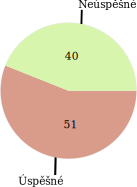
\includegraphics[width=0.28\textwidth]{../img/chart-succ.pdf}}
%     \hfill%
%     \subfloat[Graf zájmu o podobnou aplikaci.]%
%     {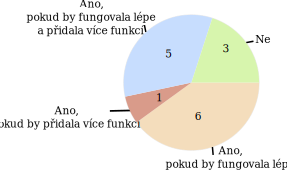
\includegraphics[width=0.6\textwidth]{../img/chart-interest.pdf}}
% \end{figure}

\newsavebox{\tempbox}
\begin{figure}[H]
    \sbox{\tempbox}{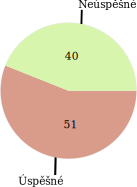
\includegraphics[width=0.28\textwidth]{../img/chart-succ.pdf}}
    \subfloat[Úspěšnost plnění.]{\usebox{\tempbox}\label{img-ratio-succ}}%
    \qquad
    \subfloat[Zájem o podobnou aplikaci.]{\vbox to \ht\tempbox{%
            \vfil
            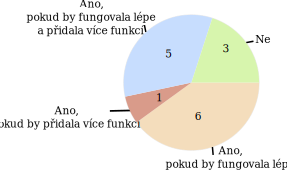
\includegraphics[width=0.6\textwidth]{../img/chart-interest.pdf}
            \vfil}\label{img-ratio-interest}}%
    \caption{Grafy výsledků.}
\end{figure}

Co se týká konkrétnějších důvodů selhání, největším problémem bylo nalezení více
kontaktů a nezdařený výběr z nich. Dalšími častými problémy bylo nerozpoznání
jména ve WA, nalezení neodpovídajících kontaktů a špatně rozpoznaná řeč.

Nutnou opravou je z pohledu uživatelů lepší rozpoznávání jmen i přiřazování
kontaktů k nim, za důležité také zmínili potvrzení vytáčení ještě jedním
\uv{ano/ne}. Několikrát byla zmíněna také plynulost aplikace a rychlost
odpovědi.
Nejvíce žádaným vylepšením byla schopnost rozpoznávat libovolný název kontaktu
místo čistě jmen, mnoho uživatelů využívá názvy kontaktů \uv{Mamka} a podobné.
Několikrát zmíněným vítaným vylepšením by také byla schopnost posílat textové
zprávy.

\section{Vylepšení a jejich možná implementace}\label{improvements}

V této sekci se budeme zabývat nutnými a možnými vylepšeními, která
vyplynula z vyhodnocení s uživateli. V podsekci~\ref{better-match}
uvedeme návrhy na zlepšení porovnávání uživatelova vstupu s jeho
seznamem kontaktů. V podsekci~\ref{better-app} pak navrhneme
úpravy v aplikaci, které by vedly k lepšímu uživatelskému
zážitku, pokud by cílem bylo čistě vytáčení kontaktů.

\subsection{Zkvalitnění přiřazování}\label{better-match}

Největším problémem bylo přiřazování názvů kontaktů spolu s neschopností přiřadit
názvy, které nejsou českými jmény. Z hlediska implementačního se o tuto část
stará WA, naše porovnávací komponenta pracuje až s entitami rozpoznanými jím.
Jako možná řešení vidíme rozšířit základnu entit, se kterými WA pracuje. Ke
každému jménu bychom mohli získat domácké formy (jako \uv{Honza} ke jménu \uv{Jan})
a přidat je do WA, kromě nich ještě běžné názvy rodinných příslušníků,
které uživatelé často využívají jako názvy kontaktů (\uv{Mamka}, \uv{Babička}).
Pro zpřesnění bychom mohli přidat i relevantní vyskloňované tvary jmen (ke jménu \uv{Jan}
také \uv{Janu}, \uv{Janovi}, \uv{Jana}).

Další možností by bylo snažit se v této omezené doméně hledat jmenné entity na
základě vzorců, když uživatel říká \uv{zavolej}, obvykle následuje název
kontaktu.

Poslední možností je přepracovat porovnávací komponentu, aby nebyla závislá
na entitách rozpoznaných pomocí WA. Touto cestou se pravděpodobně vydáme,
protože nám dává největší volnost implementace a především velkou
použitelnost mimo konkrétní doménu.

\subsection{Přepracování mobilní aplikace}\label{better-app}

Velká většina uživatelů uvedla, že by o aplikaci měli zájem, pokud by fungovala
lépe, i kdyby nepřidala další funkce. V takovém případě bychom se obešli
bez celé detekce úmyslů a mohli celý dialog velmi zjednodušit.

Navrhovaný běh představujeme v ukázce níže. Uživatel by stiskem
tlačítka zapnul rozpoznávání řeči a řekl jen název kontaktu,
kterému chce zavolat. Celý tento vstup by byl přímo v zařízení
porovnán se všemi názvy kontaktů v seznamu, pravděpodobně za
využití knihovny \texttt{JavaWuzzy}.\footnote{https://github.com/xdrop/fuzzywuzzy} Pokud by byl
nalezen jeden ostře lépe odpovídající kontakt, aplikace
by oznámila úmysl mu volat a uživatel by potvrdil \uv{ano/ne}.
Pokud by odpovídalo více kontaktů, ale méně než 4, uživatel
by z nich dostal na výběr. Pokud by jich bylo více, dostal by
žádost o zpřesnění požadavku. Celou dobu by bylo možné slovem
\uv{znovu} či obdobným začít od začátku.
\begin{code}
    Uživatel: /Stiskne tlačítko/
    Systém:   /Začne naslouchat/
    Uživatel: Název Kontaktu
    Systém:   /Porovnává celý vstup s kontakty přímo v zařízení/
    Systém:   Chcete zavolat Název Kontaktu?
    Uživatel: Ano
    Systém:   /Zahájí hovor/
\end{code}

Tím, že by celé řízení dialogu i porovnání mohlo probíhat v aplikaci,
dosáhli bychom větší plynulosti aplikace, neboť bychom nemuseli čekat
na vyřízení síťových požadavků. Zjednodušením by se celý dialog také
výrazně zrychlil, což je žádoucí, protože zahájení hovoru by mělo
být rychlé.

Ideální variantou by pak bylo kdyby i rozpoznání a generování řeči
dokázalo běžet lokálně v aplikaci bez nutnosti kontaktování serveru.
Celá aplikace by pak mohla běžet offline. Zde by mohl pomoci projekt
\texttt{DeepSpeech}.\footnote{https://github.com/mozilla/DeepSpeech}
Nutností by bylo získat dostatek trénovacích dat v češtině. Vytvořením
otevřených datasetů v mnoha jazycích se zabývá projekt Common Voice \citep{commonvoice_2020},
kam může kdokoliv dobrovolně přispět.

\chapter*{Závěr}
\addcontentsline{toc}{chapter}{Závěr}

V~kapitolách~\ref{chapter-theory}~a~\ref{chapter-wa} jsme popsali teorii nutnou
k~pochopení problematiky dialogových systémů a námi využívaného WA.
V~kapitole~\ref{chapter-implementation} jsme představili naši
implementaci dialogového systému pro hlasové vytáčení.
Nakonec v~kapitole~\ref{chapter-results} popisujeme zkušenosti
uživatelů s~naší aplíkací. Na základě zpětné vazby od nich a naší analýzy jsme navrhli možná
vylepšení systému, která jsme uvedli taktéž v~kapitole~\ref{chapter-results}.

Podařilo se nám vytvořit mobilní aplikaci pro hlasové vytáčení využívající
Google STT/TTS. Úspěšně jsme ji propojili
s~instancí WA, kterou jsme nastavili pro řízení dialogu. Ta navíc komunikuje s~námi
implementovanou porovnávací komponentou, výsledky odesíláme zpět do telefonu,
kde je případně zahájen hovor. Veškerý zdrojový kód, ukázkové video i aplikaci
připravenou k instalaci
je možné najít v přiložených souborech, které popisujeme v příloze~\ref{appendix-file}.
Kód je přístupný také online na platformě GitHub,%
\footnote{\url{https://github.com/b0r3k/dial-dial}}
zkompilovanou mobilní aplikaci pak lze stáhnout ze sekce Releases.%
\footnote{\url{https://github.com/b0r3k/dial-dial/releases/latest/download/dialog_dialer.apk}}

Naši aplikaci testovalo 15 uživatelů, kteří se dohromady pokusili zahájit 91 hovorů,
z~toho 51 úspěšně. Výsledná úspěšnost našeho systému je tedy \(56\,\rm \%\).
Jako hlavní příčinu problémů jsme identifikovali špatnou detekci entit.
Naše komponenta pracovala pouze s~entitami již alespoň částečně rozpoznanými
WA, jenže obecné rozpoznávání ve WA se ukázalo jako velmi obtížné. Jako nejlepší
řešení tedy navrhujeme změnit porovnávací komponentu, aby pracovala vždy s~celým
uživatelovým vstupem a ne jen rozšiřovala již rozpoznané entity.

Pokud bychom tuto vylepšenou komponentu z~WA volali jen při detekci uživatelova
úmyslu volat, zachovali bychom jednoduchou rozšiřitelnost aplikace. Jako
druhou možnost vidíme zaměřit se čistě na hlasové vytáčení a v~takovém
případě implementovat aplikaci s~výrazně jednodušším lokálně řízeným
dialogem, kde by i porovnávání probíhalo lokálně na celém vstupu. Ideální
variantou by bylo použít i jinou implementaci STT/TTS, pak by
celá aplikace mohla běžet offline.

Zajímavým výsledkem je, že 12 z~15 testovacích uživatelů projevilo o~podobnou
aplikaci zájem. Poukazuje to na atraktivitu hlasových asistentů
a také jejich nedostatky v~poskytování české lokalizace.

%%% Seznam použité literatury
\include{literatura}

%%% Obrázky v bakalářské práci
%%% (pokud jich je malé množství, obvykle není třeba seznam uvádět)
%\listoffigures

%%% Tabulky v bakalářské práci (opět nemusí být nutné uvádět)
%%% U matematických prací může být lepší přemístit seznam tabulek na začátek práce.
%\listoftables

%%% Použité zkratky v bakalářské práci (opět nemusí být nutné uvádět)
%%% U matematických prací může být lepší přemístit seznam zkratek na začátek práce.
\chapwithtoc{Seznam použitých zkratek}
\begin{description}
    \item[AI] Artificial Intelligence -- Umělá inteligence
    \item[API] Application Programming Interface -- Rozhraní pro programování aplikací
    \item[DA] Dialogue Act -- Dialogový akt
    \item[DST] Dialogue State Tracker -- Udržování stavu
    \item[FaaS] Function as a Service -- Funkce poskytovaná jako služba
    \item[HMM] Hidden Markov Models -- Skryté Markovovy modely
    \item[ISO] International Organization for Standardization -- Mezinárodní organizace pro normalizaci
    \item[JVM] Java Virtual Machine -- Virtuální stroj Java
    \item[MVČR] Ministerstvo vnitra České republiky
    \item[NER] Named Entity Recognition -- Rozpoznávání jmenných entit
    \item[NLU] Natural Language Understanding -- Porozumění jazyku
    \item[SDK] Software Development Kit -- Sada pro vývoj softwaru
    \item[STT] Speech to Text -- Rozpoznávání řeči
    \item[SVM] Support Vector Machines -- Metoda podpůrných vektorů
    \item[TTS] Text to Speech -- Syntéza řeči
    \item[UI] User Interface -- Uživatelské rozhraní
    \item[WA] IBM Watson Assistant
\end{description}

%%% Přílohy k bakalářské práci, existují-li. Každá příloha musí být alespoň jednou
%%% odkazována z vlastního textu práce. Přílohy se číslují.
%%%
%%% Do tištěné verze se spíše hodí přílohy, které lze číst a prohlížet (dodatečné
%%% tabulky a grafy, různé textové doplňky, ukázky výstupů z počítačových programů,
%%% apod.). Do elektronické verze se hodí přílohy, které budou spíše používány
%%% v elektronické podobě než čteny (zdrojové kódy programů, datové soubory,
%%% interaktivní grafy apod.). Elektronické přílohy se nahrávají do SISu a lze
%%% je také do práce vložit na CD/DVD. Povolené formáty souborů specifikuje
%%% opatření rektora č. 72/2017.
\appendix
\chapter{Přílohy}

\section{Přiložené soubory}\label{appendix-file}

Kód je přístupný také online na platformě GitHub,%
\footnote{\url{https://github.com/b0r3k/dial-dial}}
zkompilovanou mobilní aplikaci pak lze stáhnout ze sekce Releases.%
\footnote{\url{https://github.com/b0r3k/dial-dial/releases/latest/download/dialog_dialer.apk}}
Každá uvedená složka má vlastní soubor \texttt{README.md} s krátkým popisem.

\begin{table}[ht]

    \centering
    %%% Tabulka používá následující balíčky:
    %%%   - booktabs (\toprule, \midrule, \bottomrule)
    %%%   - dcolumn (typ sloupce D: vycentrovaná čísla zarovnaná na
    %%%     desetinnou čárku
    %%%     Všimněte si, že ve zdrojovém kódu jsou desetinné tečky, ale
    %%%     tisknou se čárky.
    %%% Dále používáme příkazy \pulrad a \mc definované v makra.tex

    %\begin{tabular}{l@{\hspace{5cm}}p{3cm}p{5cm}}
    \begin{tabular}{l@{\hspace{2cm}}p{6cm}}
        \toprule
        \textbf{Název souboru}      & \mc{\textbf{Popis}}                                      \\
        \midrule
        \texttt{dialog\_dialer.apk} & Zkompilovaná mobilní aplikace připravená k~instalaci.    \\
        \texttt{preview.mp4}        & Video demo běhu mobilní aplikace.                        \\
        \texttt{README.md}          & Krátký popis celého systému v~češtině i~angličtině.      \\
        \texttt{mobile\_app/}       & Složka se zdrojovými kódy k~mobilní aplikaci.            \\
        \texttt{watson\_init/}      & Složka se zdrojovými kódy k~nastavení WA a~získání jmen. \\
        \texttt{fuzzy\_ne/}         & Složka se zdrojovými kódy k~porovnávací komponentě.      \\
        \bottomrule
        \multicolumn{2}{l}{}
    \end{tabular}

    \label{tab-files}

\end{table}


\section{Dotazník}\label{appendix-quest}
Dotazník byl vložen samostatně a začíná na další straně.
\includepdf[pages=1-5,pagecommand={},width=\textwidth]{dotaznik.pdf}

\openright{}
\end{document}